\chapter{The geometry of two views}

Given to cameras and their projections we want to find corresponding points in the second view, given two correspondences what we can learn about the projections and restructuring the world coordinate system from correspondences.

\section{Projective geometry revisited}

\textbf{Generalizing} notion of \textbf{projective space}: $\mathbb{R}^2$ is the space of vectors with three components $0 \neq (a,b,c) \in \mathbb{R}^3$, with $\rectmat{a \\ b \\ c} = \rectmat{wa \\ wb \\ wc}, w \neq 0$. $\mathbb{R}^2$ is embedded in $\mathbb{P}^2$ by $m = (x,y) \rightarrow \hat{m} = \rectmat{x \\ y \\ 1}$.

Points in $\mathbb{P}^2$ with coordinate $c = 0$ are called \textbf{ideal points, points at infinity}.

\subsection{Describing 2D lines with projective points}

Lines in 2D space, is given by points satisfying $ax + by + c = 0$, i.e., $a,b,c$ determines the line but is \textbf{not unique}. $a,b$ are not allowed to both be zero in order to get a line.

\textbf{Normal Form}: $a^2 + b^2 = 1$, then the line is in normal form, $[a \ b]^T$ is the normal of the line and $c$ the distance to the origin.

If $\mathbf{l}$ is a line, projective coordinates on the line are: $\{\mathbf{x} \in \mathbb{P}^2 : \mathbf{x^T l} = 0\}$. We have \textbf{almost} one-to-one correspondences between lines in $\mathbb{R}^2$ and points in $\mathbb{P}^2$. What happens if $a,b$ are zero?

\textbf{This is the line at infinity:} $\mathbf{l}_\infty = \rectmat[0 \\ 0 \\ 1]$

\textbf{Useful for:} \begin{itemize}
    \item Abstract notation simplifies some calculations
    \item Some geometric relations are simpler to describe
    \item Certain special cases need not be distinguished anymore
\end{itemize}

\subsection{Intersection of two lines}

Let $\mathbf{l, l'}$ be two lines. Point of intersection: $\mathbf{x = l \times l'}$, $\times$ being the cross-product in $\mathbb{R}^3$.

\textbf{Cross-product:} $\mathbf{a,b} \in \mathbb{R}^3$, $\mathbf{a \times b} := [\mathbf{a}]_\times \mathbf{b} = \rectmat{a_2b_3-a_3b_2 \\ a_3b_1 - a_1b_3 \\ a_1b_2 - a_2 b_1}$, rule of thumb: \textbf{[23,31,12]}!

$[a]_\times = \rectmat{0 & -a_3 & a_2 \\ a_3 & 0 & -a_1 \\ -a_2 & a_1 & 0}$ is the anti-symmetric matrix of $\mathbf{a}$.

\begin{itemize}
    \item Rules can be deduced from the fact that $a \times b$ is a matrix multiplication with anti-symmetric matrix
    \item \textbf{Important rules}: {\begin{itemize}
        \item $a^T(a\times b) = b^T(a \times b) = 0$
        \item $M \in \mathbb{R}^{3\times 3}$ a transformation, them $(Ma) \times (Mb) = M^{-T} (a\times b)$
    \end{itemize}}
\end{itemize}

\subsection{Line through two points}

$\mathbf{x, x'}$ points, then $\mathbf{l = x \times x'}$ is the line that goes through both (\textbf{duality}).

\textbf{"Fun" facts:} $\mathbf{l, l'}$ both have direction $\mathbf{d}$, then their intersection is in the ideal point $\rectmat{\mathbf{d} \\ 0}$ at infinity

If $\mathbf{l}$ has direction $\mathbf{d}$, then it also intersect $\mathbf{l}_\infty$ in the ideal point.

$\mathbf{x, x'}$ ideal points, then the line that goes through both is the ideal line $\mathbf{l}_\infty$.

\subsection{Homographies of lines}

Suppose we are given $H$, what is the image of a line $\mathbf{l}$ under the homography?

Map two points to the homography and connect them $$\mathbf{l'} = (Hx \times Hx') = H^{-T} (x \times x') = H^{-T} \mathbf{l}$$, i.e. the inverse transpose of $H$.

\section{The fundamental matrix}

\subsection{Point correspondence geometry}

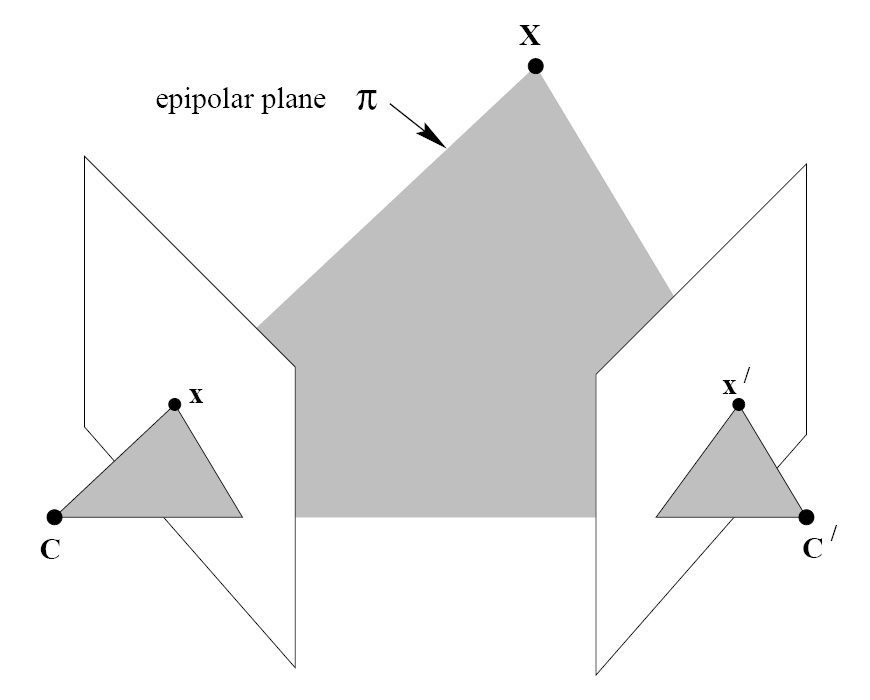
\includegraphics[width=.5\textwidth]{images/chap8/point_correspondence_geometry}

The line from $C$ to $C'$ is the \textbf{baseline}, the plane $\Pi$ containing $\mathbf{X}, C, C'$ is called \textbf{an epipolar plane}. (For each point we have one, except if they are on the same plane of course).

\textbf{Constraints on $x'$ given $x$:} \begin{itemize}
    \item $\mathbf{X}$ must lie on optic ray connecting $C$ and $\mathbf{x}$.
    \item $\mathbf{x'}$ must lie on the projection $\mathbf{l}'$ of this optic ray in $C'$
    \item This projection is called epipolar line corresponding to $\mathbf{x}$
\end{itemize}

\subsection{Epipolar planes and lines}

\begin{itemize}
    \item Baseline intersects the imageplane in epipoles $e, e'$
    \item Any plane $\Pi$ containing the baseline is an epipolar plane
    \item Intersections of $\Pi$ with the image planes are epipolar lines $l,l'$
    \item Moving a scene point $\mathbf{X}$ up or down, rotates the epipolar plane around the baseline
    \item All epipolar lines in one view, intersect at the corresponding epipole
\end{itemize}

\subsection{Fundamental matrix}

Denotes the relationship between points and their epipolar lines:

\textbf{Theorem}

Given $P, P'$, there exists $F \in \mathbb{R}^{3\times 3}$, s.t., $\mathbf{l}'$ for $\mathbf{x}$ is given by $$\mathbf{l}' = F \mathbf{x}$$, a pair of correspondences satisfies $$\mathbf{x'}^T F \mathbf{x} = 0$$,

$F$ is called the \textbf{Fundamental matrix} for the two views and can be estimated by correspondences alone.

\textbf{Properties:} \begin{itemize}
    \item $F$ for $(P,P')$, then $F^T$ for $(P',P)$ (\textbf{transpose correspondence equation)}
    \item The epipole $\mathbf{e'}$ is the left nullspace of $F$, i.e., $\mathbf{e'}^T F = 0$ and $F \mathbf{e} = 0$ (\textbf{all epilines contain the epipoles}), these equations \textbf{are used} to compute the epipoles once F is found
    \item $F$ has rank 2 (only the first two diagonal values are not zero)
    \item $F$ has \textbf{7 Degrees of Freedom}
\end{itemize}

\subsection{Computing the fundamental matrix for camera pairs}

1. Given $\mathbf{x}$ compute $\mathbf{X}_W$ which projects to $\mathbf{x}$. Using the pseudo-inverse we can find such a point using $$\mathbf{X}_W = P^+ \mathbf{x}$$

2. Project $\mathbf{X}_W$ into the second image using $P'$

3. Using the previously discussed property, we know that the epiline connects the epipole $\mathbf{e'}$ with $P'\mathbf{X}_W$, $$\mathbf{l'} = [\mathbf{e'}]_\times P' \mathbf{X}_W = \underset{=F}{\underbrace{[\mathbf{e'}]_\times P' P^+}} \mathbf{x}$$

4. The epipole $\mathbf{e'}$ is the projection of $P'C_w$ of the camera center of the first camera in world space, defined by $PC_W = 0$

\subsection{Pseudo-inverse of the projection matrix}

Using the SVD: $P^+ = V \Sigma^+ U^T$, $\Sigma^+$ constructed from $\Sigma$ taking the reciprocal of the diagonal values and then transposing the matrix. For projection matrices $n < m$ and we get $\Sigma^+$ as a right-inverse of $\Sigma$, thus $$PP^+ = U\Sigma V^T V\Sigma^+ U^T = I_3$$.

\subsection{Solutions for Fundamental matrix}

\textbf{Important} to not confuse $n<m$ and $n>m$.

$n>m$: System is over determined, usually no solution. Pseudo-inverse $\hat{x} = A^+ b$ computes $\hat{x}$ s.t. the distance from $b$ is minimized: $$\hat{x} = \mathrm{argmin} ||Ax - b||^2$$.
Pseudo-inverse finds the best approximate solution to $Ax = b$ and is a \textbf{left-inverse}.

$n<m$: Situation for the fundamental matrix. System is \textbf{under-determined}, infinitely many solutions. Pseudo-inverse $\hat{x} = A^+ b$ computes $Ax = b$ which minimizes \textbf{the norm of} $x$: $$\hat{x} = \mathrm{argmin}_{Ax = b} ||x||$$.
I.e., computes a minimum norm solution for $Ax = b$. The pseudo-inverse is a \textbf{right-inverse}.

\subsection{Summary for fundamental matrix}

For projections $P,P'$, $F = [e']_\times P' P^+$ with $e' = P'C_W$ and $PC_W = 0$. If translation and rotation parameters are known: $C_W = T^{-1} R^T \rectmat{0\\0\\0\\1}$

\subsection{Pure translational motion}

Epipole is fixed, points move along lines radiating from the epipole, hence $F = [e]_\times = [e']_\times$.

\textbf{Compact notation for a pinhole camera}: $P = K[R|t]$.

Show the previous property formally: Choose parameters $P = K[I | 0], P' = K[I | t]$. Then $P^+ = [K^{-1} \ 0]^T$ and $P'P^+ = KK^{-1} = I_3$, hence the result is \textbf{independent of translation}.

Also $C' = [-t \ 1]^T$ in world coords, thus $\mathbf{e} = K[I|0] [-t | 1]^T = -K t = Kt$ and $\mathbf{e'} = K[I|t][0 \ 1]^T = Kt$ and we have $\mathbf{e} = \mathbf{e'}$.

This way it is clear that the first statement holds.

\textbf{Horizontal motion}

Parallel to x-axis: epipole at $\mathbf{e'} = [1 \ 0 \ 0]^T$ and thus $$F = \rectmat{0 & 0 & 0\\ 0 & 0 & -1 \\ 0 & 1 & 0}$$ and the correspondence relation reduces $x' F x = 0$ to $y = y'$, along horizontal lines.

\subsection{Estimating F}
Given $n$ correspondences, for the $i$-th correspondence we get the constraint: 
$$0 = \mathbf{x'}_i F \mathbf{x}_i = [x'_i \ y'_i \ 1] \rectmat{f_{11} & f_{12} & f_{13} \\ f_{21} & f_{22} & f_{23} \\ f_{31} & f_{32} & f_{33}}[x_i \ y_i \ 1]$$ which resolves in the equation $$x_ix'_i f_{11} + y_ix'_i f_{12} +x'_i f_{13} + x_ix'_i f_{21} + y_ix'_i f_{22} + y'_i f_{23} + x_i f_{31} + y_i f_{32} + f_{33}$$ and from which we get the following system:

$$[x_ix'_i \ y_ix'_i \ x'_i \ x_iy'_i \ yiy'_i \ y'_i \ x_i \ y_i \ 1] \rectmat{f_{11} \\ f_{12} \\ f_{13} \\ f_{21} \\ f_{22} \\ f_{23} \\ f_{31} \\ f_{32} \\ f_{33} \\} = 0$$, the solution is again the rightmost column of $V$ in the SVD.

\textbf{Enforce Rank-2 constraint:} To get well-formed $F$ it must be rank 2. Compute the SVD $F' = V \Sigma V^T$ and set the last diagonal value to $0$, $F$ is then the closest to $F'$.

\textbf{Increase robustness using RANSAC:} Remove outliers using RANSAC for accurate estimation. Sufficient to estimate $F$ are \textbf{eight} sample points. "Inliers" are the feature matches satisfying the epopolar constraint given a threshold, i.e., $x' F x \leq \epsilon$.

\textbf{Summary:}

\begin{itemize}
    \item Compute feature matches (SIFT)
    \item Simple: Build large system, solve for $F$, enforce rank two constraint
    \item More robust: use RANSAC
\end{itemize}

\section{Perspective, affine and metric reconstruction}

\textbf{Projective ambiguity}: Given correspondences and assuming we reconstructed $P,P'$ and some world coordinates. Given \textbf{any} homography of the world, applying it onto the world coordinates and the projections (computing new cameras), we get the \textbf{same fundamental matrices} for the new and the old projections!

I.e., both reconstructions lead to \textbf{exactly the same correspondences}. \textbf{Mathematical limit of what we can reconstruct from correspondences alone!}

This is \textbf{projective reconstruction}.

\subsection{Affine reconstruction}

Better, as parallel lines map to parallel lines, angles are not necessarily correct.. In order to do this, we need to get rid of \textbf{projective ambiguity}. One possibility is, to identify the \textbf{plane at infinity} $\pi_\infty$.

\textbf{Plane at infinity:} Can be identified, e.g., from correspondences of \textbf{three vanishing points} detected in both images. (For instance 3 sets of parallel lines).

\subsection{Metric reconstruction}

Correct reconstruction \textbf{up to similarity} transformations (parallel lines and angles correct), but the scene might be scaled uniformly.

\textbf{Scaling ambiguity:} Segment with known absolute length must be identified (in both images).

In order to do \textbf{metric reconstruction}, we need to identify \textbf{absolute angles} (complex and not discussed!). Short: Find intrinsic parameters $K$, for which we need to compute the \textbf{Image of the Absolute Conic} (IAC), which can be described by $3\times 3$ symmetric matrix $\omega = (KK^T)^{-1}$. If $\omega$ is known, $K$ can be recovered by inverting $\omega$ and computing \textbf{Cholesky decomposition}. (The last part is not that important I guess).

\textbf{Constraints to pick from while finding $\omega$:}

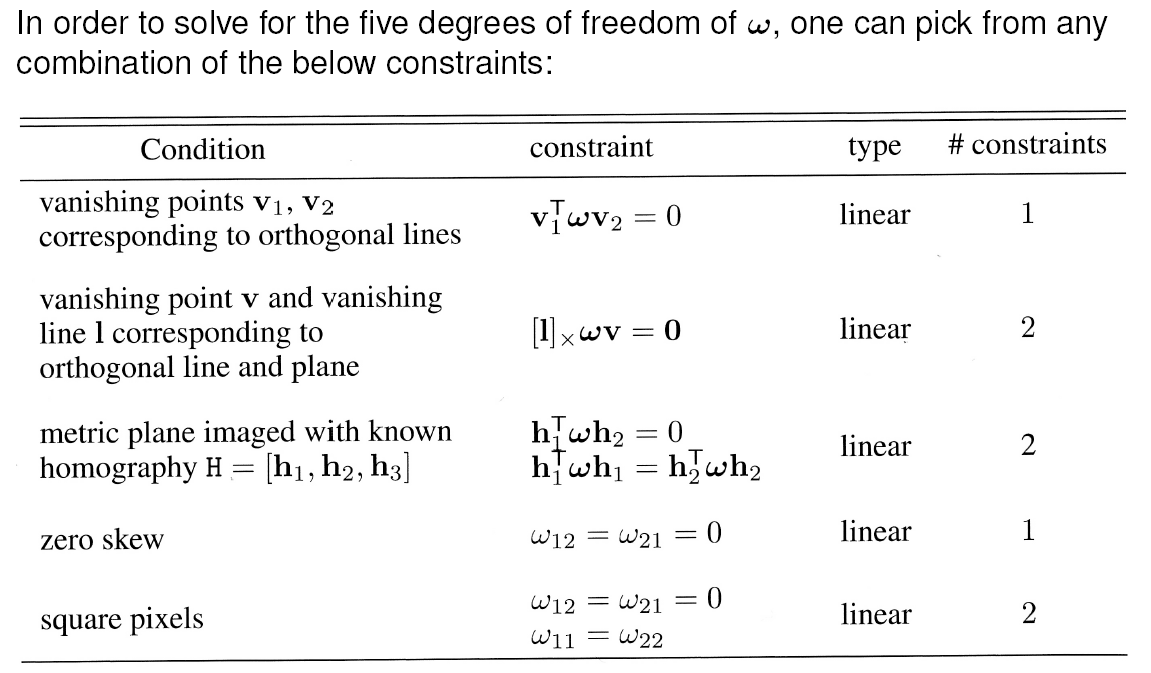
\includegraphics[width=\textwidth]{images/chap8/omega_conditions}

\section{Pose estimation : the essential matrix}

\textbf{Essential matrix:} Specialization of fundamental matrix to the pre-calibrated case where $K$ is known (hence we have \textbf{metric reconstruction}).

Under assumptions \textbf{square pixels, center of projection is center of image} we only need to calibrate the \textbf{magnification} of $K$ (focal length times pixels per meter).

\textbf{Definition:} Defined in terms of homogeneous coordinates. From a corresponding pair we get the correspondence: $$K^{-1} x = \hat{x} \leftrightarrow \hat{x}' = K'^{-1} x'$$.

The defining equation for $E$ is the correspondence constraint $\hat{x}'^T E \hat{x} = 0$. Thus, $E = K'^T F K$, and $E$ has rank two.

\textbf{Derivation from a pair of cameras:} Given a \textbf{normalized} camera pair $P = [I|0], P' = [R|t]$, we get for $E$: $$E = [e']_x P'P^+ = [[R|t][0 \ 0 \ 0 \ 1]^T]_\times [R|t][I \ 0]^T = [t]_\times R$$

Not going into detail for the decomposition..

\section{Triangulation: structure from motion}

We have two cameras $P,P'$ and correspondences. We want to find a 3D world point $PX = x$ and $P'X = x'$. Correspondence measurements usually have errors, but we can compute it (non-error free) by minimizing the \textbf{reprojection error}:

$$E(X) = \sum\limits_{i=1}^n ||PX - x||^2 + ||P'X - x'||^2$$.

\textbf{Direct linear triangulation:} $X$ can be recovered as solution to $AX = 0$:

$$A = \rectmat{x(p^3) - p^1 \\ y(p^3) - p^2 \\ x'(p'^3) - p'^1 \\ y'(p'^3) - p'^2}$$

Notes: \begin{itemize}
    \item Generalizes easily to multiple views
    \item Easy to implement
    \item Not nice mathematically: not proj. invariant
    \item Affine invariant if last coord. is forced to be zero
\end{itemize}



